\section{Differentiation of Single-Variable Functions} 

  In general, there are two ways that we define a derivative: as a limit and with infinitesimals. In a standard analysis course we use limits, but in differential equations physicists tend to use the language of infinitesimals. This is where our introduction of the hyperreals in smooth infinitesimal analysis (SIA) will be useful. 

  \begin{definition}[Derivative Using Limits]
    Given $f: [a, b] \subset \mathbb{R} \to \mathbb{R}$, fix $x \in [a, b]$, and define the \textbf{difference quotient} as the following function of $y$.\footnote{Often, textbooks introduce the difference quotient as $\frac{f(x + h) - f(x)}{h}$. These two are equivalent definitions since the following two different quotients $\phi(y) = \frac{f(x) - f(y)}{x - y}$ and $\gamma(h) = \frac{f(x + h) - f(x)}{h}$ are related in the sense that $\phi(y) = \gamma(y - x)$. So the following two limits exist simultaneously (or fail to exist simultaneously).If they do both exist, then $\lim_{y \to x} \phi(y) = \lim_{y \to x} \gamma(y - x) = \lim_{y \to 0} \gamma(y) = \lim_{h \to 0} \gamma(h)$ where the only nontrivial equality is the second equality, which is true (should be shown). }
    \begin{equation}
      \frac{f(x) - f(y)}{x - y}
    \end{equation}
    If the following limit exists, we define it's value---called the \textbf{derivative of $f$ at $x$}---as 
    \begin{equation}
      f^\prime (x) \coloneqq \lim_{y \to x} \frac{f(x) - f(y)}{x - y}
    \end{equation}
    and say $f$ is \textbf{differentiable} at $x$. If $f$ is differentiable at $x$ for every $x \in E$, then $f$ is said to be \textbf{differentiable over $E$}. 
  \end{definition} 

  So if $f$ is differentiable, we can just treat it as a new function $g(x) = f^\prime (x)$. An immediate consequence of the derivative is the following lemma, which states the existence of some error function $\varphi$ that is ``small'' in a sense. 

  \begin{lemma}[Fundamental Increment Lemma]
    Suppose the derivative of $f: [a, b] \subset \mathbb{R} \to \mathbb{R}$ at $x$ exists. Then, there exists a function $\varphi: (a, b) \subset \mathbb{R} \to \mathbb{R}$ such that 
    \begin{equation}
      f(x + h) = f(x) + f^\prime (x) h + \varphi(h) h
    \end{equation}
    for sufficiently small nonzero $h$, and 
    \begin{equation}
      \lim_{h \to 0} \varphi(h) = 0
    \end{equation}
  \end{lemma}
  \begin{proof}
    We can define 
    \begin{equation}
      \varphi(h) = \frac{f(x + h) - f(x)}{h} - f^\prime (x)
    \end{equation}
  \end{proof} 

  Is the converse is true? I think so. This gives us a new language to work with. 

  \begin{definition}[Little-O Notation]
    Let $f: \mathbb{R} \to \mathbb{R}$ be function and $g(h)$ is a monotonically increasing function with $g(0) = 0$. We say that \textbf{$f(h)$ is $o(g(h))$} if 
    \begin{equation}
      \lim_{h \to 0} \frac{f(h)}{g(|h|)} = 0
    \end{equation}
    More generally, $o(g(h))$ is a \textit{class} of functions. 
  \end{definition} 
  
  So, the $\varphi$ in the fundamental incremenent lemma is really just describing an $o(h)$ function. This is a more powerful language since we can use little-O notation to extend to other classes of functions. 

  \begin{theorem}[Differentiability with Little-o Notation]
    A function $f: [a, b] \subset \mathbb{R} \to \mathbb{R}$ is differentiable at $x$ if and only if there is a number $f^\prime (x)$ s.t. 
    \begin{equation}
      f(x + h) - f(x) = f^\prime (x) h + o(h)
    \end{equation}
    where by abuse of notation, we write $+ o(h)$ to denote adding a function in $\varphi(h) \in o(h)$.\footnote{We also use the \textit{increment notation} to write $\Delta f(x) \coloneqq f(x + h) - f(x)$ and $\Delta x \coloneqq h$ to denote the difference in the input and outputs of $f$, leading to another familiar form: $\Delta f(x) = f^\prime (x) \Delta x + o(h)$.}

    \begin{center}
        \includegraphics[scale=0.25]{img/differential_diagram.png}
    \end{center}
  \end{theorem}
  \begin{proof}
    
  \end{proof}

  In other words, the difference between the increment of the function and the value of the function $df(x)$ in $h$ is an infinitesimal of higher order than $h$. For this reason, we say that the derivative is the \textit{principal linear part of the increment of the function}. 

  In particular, if $f(x) \coloneqq x$, then we have $f^\prime (x) \coloneqq 1$ and 
  \begin{equation}
    dx (h) = 1 \cdot h = h
  \end{equation}
  Substituting this equality into $df(x) (h) = f^\prime (x) h$, we get
  \begin{equation}
    df (x) (h) = f^\prime (x) \,dx (h)
  \end{equation}
  or without the input parameter $h$, 
  \begin{equation}
    df(x) = f^\prime (x) \,dx
  \end{equation}
  Note that this is an equality between two functions of $h$. From this, we obtain the familiar \textbf{Leibniz notation} of the derivative: 
  \begin{equation}
    \frac{df (x) (h)}{dx(h)} = f^\prime (x) \iff \frac{df(x)}{dx} = f^\prime (x)
  \end{equation}
  That is, the function $\frac{df(x)}{dx}$, which is the ratio of the functions $df(x)$ and $dx$, is constant and equals $f^\prime (x)$. 

  Let us try to construct successive approximations to an arbitrary function $f: E \longrightarrow \mathbb{R}$ at a given limit point $x_0$. That is, we find a function $g$ such that
  \begin{equation}
    f = g + o(g)
  \end{equation}
  Depending on what $g$ is, we can construct better approximations of $f$. 

  \begin{example}[Constant Approximation]
    The 0th order approximation is when $g$ is a constant. That is, $g \coloneqq c_0$ for some $c_0 \in \mathbb{R}$. This means
    \begin{equation}
      f(x) = c_0 + o(c_0) = c_0 + o(1) \text{ as } x \rightarrow x_0
    \end{equation}
    More precisely, we want this difference $f(x) - c_0$ to be $o(1)$ as $x \rightarrow x_0$, which means that it is simply infinitesimal. Visualizing this, we can see that given a constant approximation (labeled in blue) to a function at $x_0$, its error term (labeled in green) is in fact, infinitesimal. All this boils down to the fact that 
    \begin{equation}
      \lim_{x \rightarrow x_0} f(x) = c_0
    \end{equation}
    If the function is continuous at $x_0$, then 
    \begin{equation}
      \lim_{x \rightarrow x_0} f(x) = f(x_0)
    \end{equation}
    and naturally $c_0 = f(x_0)$. Both the continuous (left) and noncontinuous case (right) is shown, but in most cases, we will assume continuity. 
    \begin{center}
      \includegraphics[scale=0.25]{img/constant_approximation_continuous_noncontinuous_case.png}
    \end{center}
  \end{example}

  \begin{example}[Linear Approximation]
    The 1st order approximation is a linear function that approximates $f$ as
    \begin{equation}
      f(x) = c_0 + c_1(x - x_0) + o(x - x_0) \text{ as } x \rightarrow x_0
    \end{equation}
    Following the previous logic, assuming $f$ continuous means that $c_0 = f(x_0)$. Furthermore, as $x \rightarrow x_0$
    \begin{align}
      f(x) = c_0 + c_1(x - x_0) + o(x - x_0) & \implies c_1 = \frac{f(x) - c_0 - o(x - x_0)}{x - x_0} \\
      & \implies c_1 = \frac{f(x) - c_0}{x - x_0} - \frac{o(x - x_0)}{x - x_0}\\
      & \implies c_1 = \frac{f(x) - c_0}{x - x_0} - o(1) \\
      & \implies c_1 = \lim_{x \rightarrow x_0} \frac{f(x) - c_0}{x - x_0} = f^\prime (x_0)
    \end{align}
    But this just means that $f^\prime (x_0) = c_1$, Note that before, we have proved the equivalence of the existence of a derivative at $x_0$ with differentiability at $x_0$ (which itself means that there exists a linear approximation $df(x)(h)$ that is a function of $h$). Here, we have created a linear approximation with respect to $x = x_0 + h$, rather than $h$ (shifted the function). 

    Therefore, the function 
    \begin{equation}
      \alpha (x) = f(x_0) + f^\prime (x_0) (x - x_0)
    \end{equation}
    provides the best linear approximation to the function $f$ in a neighborhod of $x_0$ in the sense that for any other function $\beta(x)$ of the form 
    \begin{equation}
      \beta(x) = c_0 + c_1 (x - x_0)
    \end{equation}
    we have $f(x) - \beta(x) \neq o(x - x_0)$ as $x \rightarrow x_0$. The graph of the function $\alpha$ is the straight line
    \begin{equation}
      y - f(x_0) = f^\prime (x_0) (x - x_0)
    \end{equation}

    This leads to the definition of our familiar tangent line. 
  \end{example}

  \begin{definition}[Tangent Line]
    If a function $f: E \longrightarrow \mathbb{R}$ is differentiable at a point $x_0 \in E$, the line defined by
    \begin{equation}
      y - f(x_0) = f^\prime (x_0) (x - x_0)
    \end{equation}
    is called the \textbf{tangent} to the graph of $f$ at the point $(x_0, f(x_0))$. 
  \end{definition}

  \begin{definition}[Tangent Space]
    Given function $f: E \longrightarrow \mathbb{R}$ and a point $x_0 \in E$, the increment of the argument $h = x - x_0$ can be regarded as a vector attached to the point $x_0$ and defining the transition from $x_0$ to $x_0 + h$. $h$ is called a \textbf{tangent vector}, and the set of all such vectors as $T_{x_0} \mathbb{R}$. Similarly, we denote $T_{y_0} \mathbb{R}$ the set of all displacement vectors from the point $y_0$ along the $y$-axis. 
    \begin{center}
        \includegraphics[scale=0.25]{img/tangent_space_1_dimensional_in_r.png}
    \end{center}
    Then, we can see that the differential is a mapping
    \begin{equation}
      df(x_0): T_{x_0} \mathbb{R} \longrightarrow T_{f(x_0)} \mathbb{R}
    \end{equation}
    Note that that there are two functions to pay attention to here: 
    \begin{enumerate}
      \item The true increment of $f$, defined $h \mapsto f(x_0 + h) - f(x_0) = \Delta f(x_0; h)$ (labeled in green). 
      \item The differential $h \mapsto f^\prime (x_0) h = df(x_0) (h)$, which gives the increment of the tangent to the graph for increment $h$ in the argument (labeled in red). 
    \end{enumerate}
  \end{definition}

  \begin{example}
    Let $f(x) = \sin{x}$. Then we will show that $f^\prime (x) = \cos{x}$. 
    \begin{align*}
        \lim_{h \rightarrow 0} \frac{\sin{(x+h)} - \sin(x)}{h} & = \lim_{h \rightarrow 0} \frac{2 \sin \big( \frac{h}{2} \big) \cos \big( x + \frac{h}{2} \big)}{h} \\
        & = \lim_{h \rightarrow 0} \cos \Big( x + \frac{h}{2} \Big) \cdot \lim_{h\rightarrow 0} \frac{\sin\big( \frac{h}{2}\big)}{\big(\frac{h}{2}\big)} = \cos(x)
    \end{align*}
    Here, we have used the theorem on the limit of a product, the continuity of the function $\cos(x)$, the equivalence $\sin{t} \sim t$ as $t \rightarrow 0$, and the theorem on the limit of a composite function. 
  \end{example}

  \begin{example}
    We will show that $\cos^\prime (x) = - \sin(x)$. 
    \begin{align*}
        \lim_{h\rightarrow 0} \frac{\cos(x+h) - \cos(x)}{h} & = \lim_{h \rightarrow 0} \frac{-2 \sin \big(\frac{h}{2}\big) \, \sin \big( x + \frac{h}{2}\big)}{h} \\
        & = - \lim_{h\rightarrow 0} \sin \Big( x + \frac{h}{2} \Big) \cdot \lim_{h\rightarrow0} \frac{\sin\big(\frac{h}{2} \big)}{\big( \frac{h}{2} \big)} = -\sin(x)
    \end{align*}
  \end{example}


  \begin{lemma}[Differentiability Implies Continuity]
    If $f$ is differentiable at $x$, it is continuous at $x$. 
  \end{lemma}
  \begin{proof} 
    If $f$ is differentiable at $x$, then the derivative 
    \begin{equation}
      f^\prime (x) = \lim_{y \to x} \frac{f(x) - f(y)}{x - y} 
    \end{equation}
    exists. Therefore, 
    \begin{align}
      0 = f^\prime (x) \cdot 0 & = f^\prime (x) \big( \lim_{y \to x} x - y \big) \\
                               & = \lim_{y \to x} \frac{f(x) - f(y)}{x - y} \cdot \lim_{y \to x} x - y \\
                               & = \lim_{y \to x} \frac{f(x) - f(y)}{x - y} (x - y) \\
                               & = \lim_{y \to x} f(x) - f(y)
    \end{align}
    which implies that $f(x) = \lim_{y \to x} f(y)$, and hence $f$ is continuous at $x$. 
  \end{proof} 

  Therefore, we can see that the set of differentiable functions is a subset of the set of continuous functions.  

\subsection{Rules of Differentiation}

  \begin{lemma}[Arithmetic]
    If $f$ and $g$ are differentiable at $x$, then 
    \begin{enumerate}
      \item $f + g$ is differentiable at $x$ with 
        \begin{equation}
          (f + g)^\prime (x) = f^\prime (x) + g^\prime (x)
        \end{equation}
      \item $fg$ is differentiable at $x$ with 
        \begin{equation}
          (fg)^\prime = f^\prime (x) g(x) + f(x) g^\prime (x)
        \end{equation}
      \item $f/g$ is differentiable at $x$ with 
        \begin{equation}
          \bigg(\frac{f}{g}) \bigg)^\prime (x) = \frac{f^\prime(x) g(x) - f(x) g^\prime (x)}{g(x)^2}
        \end{equation}
    \end{enumerate}
  \end{lemma}
  \begin{proof}
    The proof for addition is pretty trivial, so we will prove for multiplication and division. For products, let's not take the quotient just yet. 
    \begin{equation}
      (fg)(x) - (fg)(y) = f(x) g(x) - f(y) g(y) 
    \end{equation}
    We know something about $f(x) - f(y)$ and $g(x) - g(y)$, so try to put it into this form. 
    \begin{equation}
      \big(f(x) - f(y) \big) g(x) + f(y) \big( g(x) - g(y) \big)
    \end{equation}
    Therefore, 
    \begin{equation}
      \frac{(fg)(x) - (fg) (y)}{x - y} = \underbrace{\frac{f(x) - f(y)}{x - y}}_{\text{exists}} g(x) + f(y) \underbrace{\frac{g(x) - g(y)}{x - y}}_{\text{exists}}
    \end{equation}
    So by taking limits, $f$ is continuous so $f(y) \to x$ as $y \to x$, and we finally have 
    \begin{equation}
      f^\prime (x) g(x) + f(x) g^\prime (x)
    \end{equation}
    For the quotient rule, it suffices to show from the product rule that $(1/g)^\prime (x) = - \frac{g^\prime (x)}{g(x)^2}$. 
  \end{proof}

  In proving properties of differentiability, it is useful to observe that 
  \begin{equation}
    \lim_{y \to x} \frac{f(x) - f(y)}{x - y} \iff f(x) - f(y) = (x - y) (f^\prime (x) + E)
  \end{equation}
  for some function $E$ where $\lim_{y \to x} E(x) = 0$. This is known as Taylor's formula. This is similar to the decomposition of sequences into a constant plus an infinitesimal sequence. 

  From this, we can find the derivative of polynomials. 

  \begin{corollary}[Polynomial Derivatives]
    The following are true. 
    \begin{enumerate}
      \item The derivative of a constant function is $0$
      \item The derivative of the identity function $f(x) = x$ is $1$. 
      \item The derivative of $f(x) = x^n$ is $n x^{n-1}$. 
      \item The derivative of a polynomial $f(x) = a_n x^n + \ldots  + a_0$ can then be found. 
    \end{enumerate}
  \end{corollary}
  \begin{proof}
    
  \end{proof}  

  \begin{theorem}[Chain Rule]
    Let $f: [a, b] \subset \mathbb{R} \to \mathbb{R}$ be a differentiable function, fix $x \in [a, b]$, and assume differentiable $g: I \to \mathbb{R}$ where $f(x) \in I$. Then, $h = g \circ f$ is differentiable at $x$ with the derivative 
    \begin{equation}
      h^\prime (x) = g^\prime (f(x)) f^\prime (x)
    \end{equation}
  \end{theorem}
  \begin{proof}
    We have 
    \begin{equation}
      g \big( f(x)\big) - g \big( f(y)\big) = \big( f(x) - f(y) \big) \big( g^\prime (f(x)) + E_{f(y) \to f(x)}\big)
    \end{equation}
    Now we divide by $x - y$. 
    \begin{equation}
      \frac{g(f(x)) - g(f(y))}{x - y} - \frac{f(x) - f(y)}{x - y} \cdot \big( g^\prime (f(x)) + E_{f(y) \to f(x)} \big)
    \end{equation}
    Now if $x \to y$, then $f$ is continuous, which implies $f(y) \to f(x)$ and so $E \to 0$, and so by taking this limit, the above evaluates to 
    \begin{equation}
      f^\prime (x) \cdot g^\prime (f(x))
    \end{equation} 
    We could have also done 
    \begin{equation}
      \frac{g(f(x)) - g(f(y))}{x - y} = \frac{g(f(x)) - g(f(y))}{f(x) - f(y)} \cdot \frac{f(x) - f(y)}{x  - y} \to g^\prime (f(x)) \cdot f^\prime (x) 
    \end{equation}
  \end{proof}

  \begin{theorem}[Differentiation of Inverse Functions over $\mathbb{R}$]
    Let $E_1, E_2 \subset \mathbb{R}$, and $f: E_1 \longrightarrow E_2$ and $f^{-1}: E_2 \longrightarrow E_1$ be mutually inverse and continuous at points $x_0 \in E_1$ and $f(x_0) = y_0 \in E_2$. If $f$ is differentiable at $x_0$ and $f^\prime(x_0) \neq 0$, then $f^{-1}$ also differentiable at the point $y_0$, and 
    \begin{equation}
      \big(f^{-1}\big)^{-1} (y_0) = \big(f^\prime (x_0)\big)^{-1} \iff df^{-1} (y_0) = \big(df(x_0)\big)^{-1}
    \end{equation}

    \begin{figure}[H]
      \centering 
      \begin{tikzpicture}[scale=1.0]
        % Left plot - function f
        \begin{scope}
          % Axes
          \draw[->] (-1.5,0) -- (4,0) node[right] {$E_1$};
          \draw[->] (0,-1) -- (0,4) node[above] {$E_2$};
          
          % Function curve - smoother with more samples and tension
          \draw[thick] plot[domain=-1:3.5, samples=150, smooth, tension=0.9] 
              coordinates {(-1,0.5) (1,1.5) (3,4)};
          
          % Function label with direction arrow
          \node at (2.5,3.5) {$f$};
          
          % Mark point (x0, y0)
          \fill (1.5,2) circle (0.08);
          \draw[gray] (1.5,0) -- (1.5,2);
          \draw[gray] (0,2) -- (1.5,2);
          \node[below] at (1.5,0) {$x_0$};
          \node[left] at (0,2) {$y_0$};
          
          % Tangent line at (x0, y0)
          \draw[blue, thick, ->] (0,0.5) -- (3,3.5);
          \node[blue] at (3.5,2.5) {$f'(x_0)$};
        \end{scope}
        
        % Right plot - inverse function f^{-1}
        \begin{scope}[xshift=8cm]
          % Axes
          \draw[->] (-1.5,0) -- (4,0) node[right] {$E_2$};
          \draw[->] (0,-1) -- (0,4) node[above] {$E_1$};
          
          % Inverse function curve
          \draw[thick] plot[domain=-1:3.5, samples=100, smooth] 
              coordinates {(0.5, -1) (1.5, 1) (4, 3)};
          
          % Function label with direction arrow
          \node at (3.5,2) {$f^{-1}$};
          
          % Mark point (y0, x0)
          \fill (2,1.5) circle (0.08);
          \draw[gray] (2,0) -- (2,1.5);
          \draw[gray] (0,1.5) -- (2,1.5);
          \node[below] at (2,0) {$y_0$};
          \node[left] at (0,1.5) {$x_0$};
          
          % Tangent line at (y0, x0)
          \draw[blue, thick, ->] (0.5,0) -- (3.5,3);
          \node[blue] at (0.5,2.5) {$(f^{-1})'(x_0)=\frac{1}{f'(x_0)}$};
        \end{scope}
      \end{tikzpicture}
      \caption{Relationship between a function $f$ and its inverse $f^{-1}$, showing how their derivatives are related}
      \label{fig:function-inverse}
    \end{figure}

    Note that if we knew in advance that $f^{-1}$ was differentiable at $y_0$ (which is a stronger hypothesis), we can find immediately by the identity 
    \begin{equation}
      (f^{-1} \circ f) (x) = x
    \end{equation}
    and the theorem on the differentiation of a composite function that
    \begin{equation}
      (f^{-1})^\prime (y_0) \cdot f^\prime (x_0) = 1
    \end{equation}
  \end{theorem}

  Note that if the hypothesis was satisfied, but $f^\prime (x_0) = 0$, then $f^{-1}$ would not be differentiable since it would have an undefined differential. 

  \begin{figure}[H]
    \centering 
    \begin{tikzpicture}[scale=1.3]
      % Left plot - function f with three points
      \begin{scope}
        % Axes
        \draw[->] (-2,0) -- (2,0) node[right] {$x$};
        \draw[->] (0,-2) -- (0,2) node[above] {$y$};

        \draw[<->, blue] (-1,1) -- (1,1) node[above] {$f^\prime (x_0) = 0$};
        
        % Connect the points with a smooth curve
        \draw[thick] plot[smooth, tension=0.9] coordinates {(-1,0) (0,1) (1,0)};
        
        % Function label
        \node at (0.5,0.2) {$f$};
      \end{scope}
      
      % Right plot - inverse function
      \begin{scope}[xshift=6cm]
        % Axes
        \draw[->] (-2,0) -- (2,0) node[right] {$y$};
        \draw[->] (0,-2) -- (0,2) node[above] {$x$};
        \draw[<->, blue] (1,-1) -- (1,1) node[right] {$(f^{-1})^\prime (x_0) = ?$};
        
        % Connect the points with a smooth curve (same tension)
        \draw[thick] plot[smooth, tension=0.9] coordinates {(0,-1) (1,0) (0,1)};
        
        % Function label
        \node at (0.2,0.5) {$f^{-1}$};
      \end{scope}
    \end{tikzpicture}
    \caption{A function through three points and its inverse relation}
    \label{fig:three-point-function-inverse}
  \end{figure}

\subsection{Theorems of Differentiable Functions}

  \begin{theorem}[Local Extrema of Differentiable Functions Have Vanishing Derivative]
    Let $f: [a, b] \to \mathbb{R}$ and assume $f$ has a local maximum at $c \in (a, b)$ with $f$ differentiable at $c$. Then $f^\prime (c) = 0$. 
  \end{theorem}
  \begin{proof}
    Let us pick two sequences---a left one and a right one---that converges to $x$ from either side. 
    \begin{enumerate}
      \item If $x > c$ (with $x$ sufficiently close to $c$), then $f(c) \geq f(x)$ and so 
      \begin{equation}
        \frac{f(c) - f(x)}{c - x} \leq 0 \implies f^\prime (c) = \lim_{c - x} \frac{f(c) - f(x)}{c - x} \leq 0
      \end{equation}

      \item If $x < c$, then $f(c) \geq f(x)$ and so 
      \begin{equation}
        \frac{f(c) - f(x)}{c - x} \geq 0 \implies f^\prime (c) = \lim_{c - x} \frac{f(c) - f(x)}{c - x} \geq 0
      \end{equation}
    \end{enumerate}
    So $0 \leq f^\prime (c) \leq 0 \implies f^\prime(c) = 0$. 
  \end{proof}

  Note that it is generally not true that $f^\prime (c) = 0$ if $c = a$ or $c = b$, i.e. at the endpoints. 

  \begin{theorem}[Rolle's Theorem]
    Suppose $f: [a, b] \to \mathbb{R}$ is differentiable on $(a, b)$. Then, if $f(a) = f(b)$, then there exists a $c \in (a, b)$ such that $f^\prime (c) = 0$. 
  \end{theorem}
  \begin{proof}
    Since $f$ is continuous on $[a, b]$, it has to attain its global max and min values somewhere in $[a, b]$. If either is in $(a, b)$, then the derivative is $0$. If max and min are attained on $\{a, b\}$, then since $f(a) = f(b)$, this implies that $f(x) = f(a)$ for all $x \in [a, b]$, which implies $f^\prime (x) = 0$. 
  \end{proof}

  \begin{theorem}[Mean Value Theorem]
    Assume $f: [a, b] \to \mathbb{R}$ is differentiable. Then there exists a $c \in (a, b)$ for which 
    \begin{equation}
      f^\prime (c) = \frac{f(b) - f(a)}{b - a} \iff f^\prime (c) (b - a) = f(b) - f(a)
    \end{equation}
  \end{theorem}
  \begin{proof}
    Just use Rolle's on 
    \begin{equation}
      g(x) = f(x) - \bigg[ \frac{f(b) - f(a)}{b - a} (x - a) + f(a) \bigg]
    \end{equation}
    which satisfies $g(a) = g(b) = 0$, and so there must exist some $c \in (a, b)$ such that $g^\prime (c) = 0$, i.e. 
    \begin{equation}
      f^\prime (c) - \frac{f(b) - f(a)}{b - a} = 0 \implies f^\prime (c) = \frac{f(b) - f(a)}{b - a}
    \end{equation}
  \end{proof} 

  Geometrically, this means that there exists a tangent line somewhere at $\zeta \in (a, b)$ that is parallel the secant line connecting the two points $\big(a, f(a)\big)$ and $\big( b, f(b)\big)$. 

  Some remarks: 
  \begin{enumerate}
    \item Physically, if $x$ is interpreted as time and $f(b) - f(a)$ as the amount of displacement over the time $b-a$ of a particle moving along the line, this theorem says that the velocity $f^\prime (x)$ of the particle at some time $\zeta \in (a, b)$ is such that if the particle had moved with constant velocity $f^\prime (\zeta)$ over the whole time interval, it would have been displaced by the same amount $f(b) - f(a)$. We call $f^\prime (\zeta)$ the \textbf{average velocity} over the time interval $[a, b]$. 
    \item Note that the Mean Value Theorem is important in that it connects the increment of a function over a finite interval with the derivative of the function on that interval. Up to now, we have characterized only the local (infinitesimal) increment of a function in terms of the derivative or differential at a given point. MVT connects the increment of a function over a \textbf{finite} interval with the derivative of the function. 
  \end{enumerate}

  The MVT actually leads to multiple useful corollaries. 

  \begin{theorem}[Derivative of a Monotonic Function]
    Given function $f: [a, b] \longrightarrow \mathbb{R}$ that is differentiable on $(a, b)$, 
    \begin{align*}
      f^\prime (x) > 0 & \implies f \text{ is increasing} \\
      f^\prime (x) \geq 0 & \iff f \text{ is nondecreasing} \\
      f^\prime (x) \coloneqq 0 & \iff f \text{ is constant} \\
      f^\prime (x) \leq 0 & \iff \text{ is nonincreasing} \\
      f^\prime (x) < 0 & \implies f \text{ is decreasing} 
    \end{align*}
    Note the one-sided direction for the strict inequalities.\footnote{Think of the function $f(x) = x^3$, which is strictly increasing, but has derivative $f^\prime (0) = 0$ at $x = 0$.} The reverse implication is a bit weaker. 
    \begin{align*}
      f \text{ is increasing} & \implies f^\prime (x) \geq 0 \\
      f \text{ is decreasing} & \implies f^\prime (x) \leq 0
    \end{align*}
  \end{theorem}
  \begin{proof}
    If $x_1 < x_2$ are two points of the interval, then the MVT
    \begin{equation}
      f(x_2) - f(x_1) = f^\prime (\zeta) (x_2 - x_1)
    \end{equation}
    shows that the sign of the left hand side must equal that of the right. 
  \end{proof}

  \begin{corollary}[Derivative of a Constant Function]
    A function that is continuous on a closed interval $[a,b]$ is constant on it if and only if its derivative equals $0$ at every point of the interval $[a,b]$ or the open interval $(a, b)$. 

    Therefore, if the derivatives $f_1^\prime (x)$ and $f_2^\prime (x)$ of two functions $f_1 (x)$ and $f_2 (x)$ are equal on some interval (that is, $f_1^\prime (x) = f_2^\prime (x)$ on the interval), then the difference
    \begin{equation}
      (f_1 - f_2) (x) = f_1 (x) - f_2 (x)
    \end{equation}
    is constant. 
  \end{corollary}
  \begin{proof}
    Given constant function $f$, the MVT equation 
    \begin{equation}
      0 = f(x_2) - f(x_1) = f^\prime (\zeta) (x_2 - x_1)
    \end{equation}
    implies that $f^\prime (\zeta) = 0$ for all $x_1, x_2 \in E$. It follows that by the arithmetic properties of the derivative, given two functions $f_1, f_2$ with the same derivative on an interval, the derivative of their difference $(f_1 - f_2)^\prime = 0$, and therefore must be constant on that interval. 
  \end{proof}

  \begin{theorem}[IVT For Derivatives]
    Suppose $f: [a, b] \to \mathbb{R}$ is a real and differentiable function and suppose $f^\prime (a) < \lambda < f^\prime (b)$. Then there exists $x \in (a, b)$ such that $f^\prime (x) = \lambda$.\footnote{i.e. $f$ doesn't have to be continuous, but it must have a middle value.}
  \end{theorem}
  \begin{proof}
    Let $g(x) = f(x) - \lambda x$. Then $g$ is differentiable with $g^\prime (x) = f^\prime (x) - \lambda$. But this implies that
    \begin{enumerate}
      \item $g^\prime (a) = f^\prime (a) - \lambda < 0$, which implies that 
      \begin{equation}
        \frac{g(t_1) - g(a)}{t_1 - a} < 0 \implies g(t_1) - g(a) < 0 \implies g(t_1) < g(a)
      \end{equation}
      for some $t_1 > a$ sufficiently close to $a$. 

      \item $g^\prime (b) = f^\prime (b) - \lambda > 0$, which implies that 
      \begin{equation}
        \frac{g(t_2) - g(b)}{t_2 - b} > 0 \implies g(t_2) - g(b) > 0 \implies g(t_2) > g(b)
      \end{equation}
      for some $t_2 < b$ sufficiently close to $b$. 
    \end{enumerate}
    By the mean value theorem there exists $x \in (a, b)$ s.t. $g^\prime (x) = 0 \implies f^\prime (x) = \lambda$. 
  \end{proof}

  \begin{corollary}[Derivatives Cannot Have Jump Discontinuities]
    You can't have a jump discontinuity\footnote{Also called a discontinuity of the first kind.} for derivatives. 
  \end{corollary}

  That is, the derivative of a differentiable function cannot ``jump,'' so it's like the IVT of derivatives. However, it may as well have discontinuities of the second kind. 

  \begin{example}[Derivative Might Jump if Not Differentiable]
    A non-example is $f(x) = |x|$. It is not differentiable over $[-1, 1]$, and so we see a jump in the derivative. 
  \end{example}

  The following theorem is a useful generalization of Lagrange's theorem. 

  \begin{theorem}[Cauchy's Finite-Increment Theorem]
    Let $x = x(t)$ and $y = y(t)$ be functions that are continuous on a closed interval $[\alpha, \beta]$ and differentiable on the open interval $(\alpha, \beta)$. Then, there exists a point $\tau \in [\alpha, \beta]$ such that
    \begin{equation}
      x^\prime (\tau) \big( y(\beta) - y (\alpha)\big) = y^\prime (\tau) \big( x(\beta) - x(\alpha)\big)
    \end{equation}
    If in addition $x^\prime (t) \neq 0$ for each $t \in (\alpha, \beta)$, then $x(\alpha) \neq x(\beta)$ and we have the equality 
    \begin{equation}
      \frac{y(\beta) - y(\alpha)}{x(\beta) - x(\alpha)} = \frac{y^\prime (\tau)}{x^\prime (\tau)}
    \end{equation}
  \end{theorem}

\subsection{Extrema and Concavity}

  Similarly, we can connect the concepts of extrema and derivatives. 

  \begin{theorem}[First Derivative Test]
    Let function $f: E \longrightarrow \mathbb{R}$ be defined in a neighborhood $U(x_0)$ of point $x_0$, which is continuous at $x_0$ and differentiable in $\mathring{U}(x_0)$, a deleted neighborhood of $x_0$. (Note that this is broader hypothesis than just assuming that $f$ be differentiable at $x_0$.) Let
    \begin{equation}
      \mathring{U}^- (x_0) \coloneqq \{x \in U(x_0) \;|\; x < x_0\}, \;\; \mathring{U}^+ (x_0) \coloneqq \{x \in U(x_0) \;|\; x > x_0\}
    \end{equation}
    That is, $\mathring{U}^- (x_0)$ is the left portion of $\mathring{U}(x_0)$ and $\mathring{U}^+ (x_0)$ is the right portion of $\mathring{U}(x_0)$. Then, 
    \begin{enumerate}
      \item $(x_0, f(x_0))$ is strict local minimum if $f^\prime(x) < 0$ in $\mathring{U}^- (x_0)$ and $f^\prime (x) > 0$ in $\mathring{U}^+ (x_0)$. 

      \item $(x_0, f(x_0))$ is strict local maximum if $f^\prime(x) > 0$ in $\mathring{U}^- (x_0)$ and $f^\prime (x) < 0$ in $\mathring{U}^+ (x_0)$. 

      \item $(x_0, f(x_0))$ has no extremum at $x_0$ if $f^\prime (x) > 0$ in both $\mathring{U}^- (x_0), \mathring{U}^+ (x_0)$, or if $f^\prime(x)< 0$ in both $\mathring{U}^- (x_0), \mathring{U}^+ (x_0)$. 
    \end{enumerate}
  \end{theorem}

  Note that if there is a discontinuity at a point $x_0$, then this theorem does not apply. For example, $(x_0, f(x_0))$ in the graph below is a local minimum, even though the derivatives to the left of $x_0$ are positive and those to the right of $x_0$ are negative (within neighborhood $U(x_0)$). Similarly, $(x_0, g(x_0))$ is a local maximum, even though the derivative to the left and to the right of $x_0$ are both positive. 
  \begin{center}
      \includegraphics[scale=0.3]{img/theorem_not_apply_if_discontinuity.png}
  \end{center}

  \begin{theorem}[2nd, $n$th Derivative Test]
    Let function $f: E \longrightarrow \mathbb{R}$ be defined on a neighborhood $U(x_0)$ of $x_0$ has derivatives of order up to $n$ inclusive at $x_0$. If its derivatives up to the $(n-1)$th order vanishes 
    \begin{equation}
      f^\prime (x_0) = f^{\prime\prime} (x_0) ... = f^{(n-1)} (x_0) = 0
    \end{equation}
    but the $n$th derivative at $x_0$ does \textbf{not} vanish
    \begin{equation}
      f^{(n)} (x_0) \neq 0
    \end{equation}
    then 
    \begin{enumerate}
      \item $n$ is odd $\implies$ there is no local extremum at $x_0$ 
      \item $n$ is even $\implies$ there is a local extremum at $x_0$
      \begin{enumerate}
        \item $f^{(n)} (x_0) > 0 \implies$ it is a strict local minimum
        \item $f^{(n)} (x_0) < 0 \implies$ it is a strict local maximum
      \end{enumerate}
    \end{enumerate}
  \end{theorem}

  \begin{definition}[Convex, Concave Functions]
    A function $f: (a, b) \longrightarrow \mathbb{R}$ defined on an open interval $(a, b) \subset \mathbb{R}$ is \textbf{convex} if the inequality
    \begin{equation}
      f( \alpha_1 x_1 + \alpha_2 x_2) \leq \alpha_1 f(x_1) + \alpha_2 f(x_2)
    \end{equation}
    holds and \textbf{concave}, or \textbf{convex upward}, if the inequality 
    \begin{equation}
      f( \alpha_1 x_1 + \alpha_2 x_2) \geq \alpha_1 f(x_1) + \alpha_2 f(x_2)
    \end{equation}
    holds for all pairs of points $x_1, x_2 \in (a, b)$ and any numbers $\alpha_1, \alpha_2 \geq 0$ such that $\alpha_1 + \alpha_2 = 1$. If this inequality is strict whenever $x_1 \neq x_2$ and $\alpha_1 \alpha_2 \neq 0$, the function is said to be \textbf{strictly convex} and \textbf{strictly concave}, respectively. 
  \end{definition}

  Note that using induction on the number of points, we get a primitive form of Jensen's inequality. 

  \begin{lemma}[Jensen's Inequality]
    If $f: (a, b) \longrightarrow \mathbb{R}$ is a convex function, $x_1, ..., x_n$ are points of $(a, b)$, and $\alpha_1, ..., \alpha_n$ are nonnegative numbers such that $\alpha_1 + ... + \alpha_n = 1$, then 
    \begin{equation}
      f(\alpha_1 x_1 + ... + \alpha_n x_n) \leq \alpha_1 f(x_1) + ... + \alpha_n f(x_n)
    \end{equation}
  \end{lemma}

  The following is also another equivalent condition for a function to be convex over $(a, b)$. 

  \begin{theorem}
    A function $f: (a, b) \longrightarrow \mathbb{R}$ that is differentiable on the open interval $(a, b)$ is convex on $(a, b)$ if and only if its graph contains no points below any tangent drawn to it.
  \end{theorem}

  \begin{theorem}[2nd Derivatives of Convex Functions]
    Given a function $f: (a, b) \longrightarrow \mathbb{R}$ that is differentiable in its domain, 
    \begin{enumerate}
      \item $f$ is convex $\iff f^\prime$ is nondecreasing on $(a, b) \iff f^{\prime\prime} \geq 0$ on $(a, b)$ 
      \item $f$ is strictly convex $\iff f^\prime$ is increasing on $(a, b) \iff f^{\prime\prime} > 0$ on $(a, b)$ 
      \item $f$ is concave $\iff f^\prime$ is nonincreasing on $(a, b) \iff f^{\prime\prime} \leq 0$ on $(a, b)$ 
      \item $f$ is strictly concave $\iff f^\prime$ is decreasing on $(a, b) \iff f^{\prime\prime} < 0$ on $(a, b)$ 
    \end{enumerate}
  \end{theorem}

  \begin{definition}[Inflection Point]
    Let $f: E \longrightarrow \mathbb{R}$ be a function defined and differentiable on a neighborhood $U(x_0)$. If the function is convex downward (resp. upward) on the set $\mathring{U}^- (x_0) = \{x \in U(x_0) \;|\; x < x_0\}$ and convex upward (resp. downward) on $\mathring{U}^+ (x_0) = \{x \in U(x_0)\;|\; x > x_0\}$, then the point 
    \begin{equation}
      \big( x_0, f(x_0) \big)
    \end{equation}
    is called a \textbf{inflection point of the graph}. 

    \begin{figure}[H]
      \centering 
      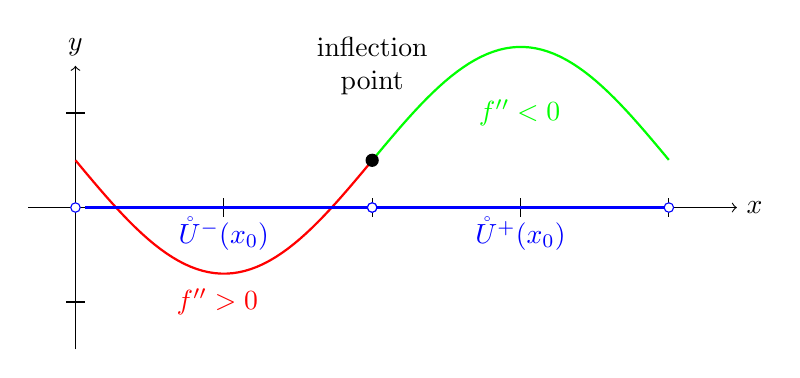
\begin{tikzpicture}[scale=1.2]
        % Draw coordinate axes
        \draw[->] (-0.5,0) -- (7,0) node[right] {$x$};
        \draw[->] (0,-1.5) -- (0,1.5) node[above] {$y$};
        
        % Draw the negative sine curve in two colors, shifted up by 0.5
        \draw[thick, red] plot[domain=0:3.14, samples=50] (\x, {-sin(\x r) * 1.2 + 0.5});
        \draw[thick, green] plot[domain=3.14:6.28, samples=50] (\x, {-sin(\x r) * 1.2 + 0.5});
        
        % Add second derivative labels
        \node[red] at (1.5,-1) {$f^{\prime\prime} > 0$};
        \node[green] at (4.7,1) {$f^{\prime\prime} < 0$};
        
        % Add inflection point label - updated y-coordinate to match the shift
        \fill (3.14,0.5) circle (0.07);
        \node[align=center] at (3.14,1.5) {inflection\\point};
        
        % Add key points on x-axis (ticks only, no labels)
        \foreach \x in {0, 1.57, 3.14, 4.71, 6.28} {
          \draw (\x,0.1) -- (\x,-0.1);
        }
        
        % Add blue intervals with hollow endpoints
        % First interval (0, pi)
        \draw[blue, thick] (0.1,0) -- (3.14,0);
        \draw[blue, fill=white] (0.0,0) circle (0.05);
        \draw[blue, fill=white] (3.14,0) circle (0.05);
        \node[blue, below] at (1.57,0) {$\mathring{U}^{-}(x_0)$};
        
        % Second interval (pi, 2pi)
        \draw[blue, thick] (3.14,0) -- (6.28,0);
        \draw[blue, fill=white] (3.14,0) circle (0.05);
        \draw[blue, fill=white] (6.28,0) circle (0.05);
        \node[blue, below] at (4.71,0) {$\mathring{U}^{+}(x_0)$};
        
        % Add key points on y-axis (ticks only, no labels)
        \foreach \y in {-1, 1} {
          \draw (0.1,\y) -- (-0.1,\y);
        }
      \end{tikzpicture}
      \caption{Curve with changing concavity and inflection point at $\pi$}
      \label{fig:neg-sine-concavity}
    \end{figure}
  \end{definition}

\subsection{Theorems of Continuously Differentiable Functions}

  Now continuously differentiable functions are called \textit{smooth functions}, denoted $f \in C^1([a, b])$. 

  \begin{theorem}[$C^1$ Implies Lipschitz]
    A continuously differentiable function is Lipschitz continuous. 
  \end{theorem}
  \begin{proof}
    
  \end{proof} 

  \begin{example}
    Suppose $f$ is twice-differentiable on $\mathbb{R}$ and that $M_0, M_1, M_2$ are the least upper bounds of $|f(x)|$, $|f^\prime (x)|$, and $|f^{\prime\prime} (x)|$. Then $M_1^2 \leq 4 M_0 M_2$. 


  \end{example}

  \begin{theorem}[L'Hopital's Rule]
    Suppose $f, g$ are continuously differentiable functions with $f(c) = g(c) = 0$ and $g^\prime (c) \neq 0$. Then, 
    \begin{equation}
      \lim_{x \to c} \frac{f(x)}{g(x)} = \lim_{x \to c} \frac{f^\prime (x)}{g^\prime (x)}
    \end{equation}
  \end{theorem}
  \begin{proof}
    We have 
    \begin{align}
      \lim_{x \to c} \frac{f(x)}{g(x)} & = \lim_{x \to c} \frac{f(x) - f(c)}{g(x) - g(c)} \\ 
                                       & = \lim_{x \to c} \frac{\frac{f(x) - f(c)}{x -  c}}{\frac{g(x) - g(c)}{x - c}} \\ 
                                       & = \frac{\lim_{x \to c} \frac{f(x) - f(c)}{x - c}}{\lim_{x \to c} \frac{g(x) - g(c)}{x - c}} \\ 
                                       & = \lim_{x \to c} \frac{f^\prime (x)}{g^\prime (x)}
    \end{align}
  \end{proof}

  \begin{example}
    Let $f(x) = \sin{x}$ and $g(x) = -0.5x$. Then, the function 
    \begin{equation}
      h(x) = \frac{f(x)}{g(x)} = \frac{\sin{x}}{-0.5x}
    \end{equation}
    is clearly undefined at $x = 0$. 
    However, we can solve the limit using L'Hopital's rule to get
    \begin{equation}
      \lim_{x \rightarrow 0} \frac{\sin{x}}{-0.5x} = \lim_{x \rightarrow 0} \frac{\cos{x}}{-0.5} = -2
    \end{equation}
    Therefore, $h: \mathbb{R} \setminus 0 \longrightarrow \mathbb{R}$ can be completed to continuous function on all of $\mathbb{R}$ by defining the extension: 
    \begin{equation}
      H(x) \coloneqq \begin{cases} h(x), & x \neq 0 \\ -2, & x = 0 \end{cases} 
    \end{equation}
  \end{example}

\subsection{Higher Order Derivatives} 

  Note that the mean value theorem states that given differentiable $f: [a, b] \to \mathbb{R}$, there exists a $c \in (a, b)$ s.t. 
  \begin{equation}
    f (b) = f (a) + f^\prime (c) (b - a) 
  \end{equation}
  which is like a first order approximation. We would like to attain a second order approximation using the fact that $f$ is twice differentiable. To do this, recall how we proved the MVT. We subtracted a linear function from $f(x)$ to get a new function $g(x)$ satisfying $g(a) = g(b) = 0$. We will do the same here.

  \begin{theorem}[Taylor's Theorem of 2nd Order]
    If $f$ is twice differentiable on $[a, b]$, then 
    \begin{equation}
      f(b) = f(a) + f^\prime (b) (b - a) + \frac{f^{\prime \prime}(c)}{2} (b-a)^2
    \end{equation}
    for some $c \in (a, b)$. This is like a mean value theorem for the second order, where only the final term is dependent on $c$. 
  \end{theorem} 
  \begin{proof}
    Let us define the function 
    \begin{equation}
      g(x) \coloneqq f(x) - f(a) - f^\prime (a) (x - a) - M (x - a)^2
    \end{equation} 
    where $M$ was chosen such that $g(b) = 0$. Now notice that 
    \begin{align}
      g(a) & = f(a) - f(a) - 0 - 0 = 0 \\ 
      g^\prime (a) & = f^\prime (a) - f^\prime (a) - 0 = 0 
    \end{align}
    and so by using Rolle's theorem on $g$, there exists a $c_1 \in (a, b)$ s.t. 
    \begin{equation}
      g^\prime (c_1) (b - a) = g(b) - g(a) = 0 - 0 = 0 \implies g^\prime (c_1) = 0
    \end{equation}  
    therefore, we can use Rolle's theorem again on $g^\prime$ and claim there exists a $c \in (a, c_1)$ s.t. 
    \begin{equation}
      g^{\prime\prime} (c) (c_1 - a) = g^\prime (c_1) - g^\prime (a) = 0 - 0 = 0 \implies g^{\prime\prime} (c) = 0
    \end{equation}
    This gives us all we need. By taking the double derivative of $g$, we get 
    \begin{equation}
      0 = g^{\prime\prime} (c) = f^{\prime\prime} (c) - 2M \implies M = \frac{f^{\prime\prime} (c)}{2}
    \end{equation}
    and substituting this in gives 
    \begin{equation}
      0 = g(b) = f(b) - f(a) - f^\prime (a) (b - a) - \frac{f^{\prime\prime} (c)}{2} (b - a)^2
    \end{equation}
  \end{proof}

  We can continue this process to get a $n$th order approximation. 

  \begin{theorem}[Taylor's Theorem]
    Suppose $f: [a, b] \to \mathbb{R}$, is $n$th differentiable over $[a, b]$ and $f^{(n+1)}$ exists over $(a, b)$. Then there exists a $c \in (a, b)$ s.t. 
    \begin{equation}
      f(b) = \bigg( \sum_{k=0}^n \frac{f^{(k)}(a)}{k!} (b - a)^k  \bigg) + \frac{f^{(n+1)} (c)}{(n+1)!} (b - a)^{n+1}
    \end{equation} 
    Where 
    \begin{equation}
      \varepsilon_f \coloneqq 
    \end{equation}
  \end{theorem}
  \begin{proof}
    We do the exact same process. Let us define 
    \begin{equation}
      P(x) = \sum_{k=0}^n \frac{f^{(k)} (a)}{k!} (x - a)^k
    \end{equation} 
    and set 
    \begin{equation}
      g(x) \coloneqq f(x) - P(x) - M (x - a)^{n+1}
    \end{equation} 
    where $M$ was chosen such that $g(b) = 0$. Now notice that evaluating on $g$ gives us 
    \begin{equation}
      g(a) = g^\prime (a) = g^{\prime\prime} (a) = \ldots = g^{(n)} (a) = 0 
    \end{equation} 
    So by using Rolle's theorem on $g$, there exists a $c_1 \in (a, b)$ s.t. $g^\prime (c_1) = 0$. Therefore we can use Rolle's theorem on $g^\prime$ to show there exists a $c_2 \in (a, c_1)$. We keep doing this until we show that there exists a $c \in (a, b)$ s.t. $g^{(n)} (c) = 0$. With this, we can directly evaluating the $n$th derivative of $g$ to find 
    \begin{equation}
      0 = g^{(n)} (c) = f^{(n)} (c) - n! M \implies M = \frac{f^{(n)} (c)}{n!}
    \end{equation}
  \end{proof}

  We can continue this pattern to get a quadratic approximation of $f$ in the form
  \begin{equation}
    f(x) = c_0 + c_1 (x - x_0) + c_2 (x - x_0)^2 + o\big((x - x_0)^2 \big) \text{ as } x \rightarrow x_0
  \end{equation}
  As we have done in the previous subsection, we can derive (assuming continuity of $f$) $c_0 = f(x_0), c_1 = f^\prime (x_0)$. To derive what $c_2$ should be, we see that the equation above implies
  \begin{equation}
    c_2 = \frac{f(x) - c_0 - c_1 (x - x_0) - o\big((x - x_0)^2 \big)}{(x - x_0)^2} = \frac{f(x) - c_0 - c_1 (x - x_0)}{(x - x_0)^2} - o(1)
  \end{equation}
  which means
  \begin{equation}
    c_2 = \lim_{x \rightarrow x_0} \frac{f(x) - c_0 - c_1 (x - x_0)}{(x - x_0)^2}
  \end{equation}
  Extending this, if we are seeking a polynomial $P_n(x_0; x) = c_0 + c_1 (x - x_0) + \ldots + c_n (x - x_0)^n$ such that
  \begin{equation}
    f(x) = c_0 + c_1 (x - x_0) + \ldots + c_n (x - x_0)^n + o\big((x - x_0)^n\big) \text{ as } x \rightarrow x_0
  \end{equation}
  we would find 
  \begin{align}
      c_0 & = \lim_{x \rightarrow x_0} f(x) \\
      c_1 & = \lim_{x \rightarrow x_0} \frac{f(x) - c_0}{x - x_0} \\
      c_2 & = \lim_{x \rightarrow x_0} \frac{f(x) - c_0 - c_1 (x - x_0)}{(x - x_0)^2} \\
      \ldots & = \ldots \\
      c_n & = \lim_{x \rightarrow x_0} \frac{f(x) - (c_0 + \ldots + c_{n-1}(x - x_0)^{n-1})}{(x - x_0)^n}
  \end{align}

  We formalize the order of these approximations by analyzing their error bound. 

  \begin{definition}[nth Order Contact]
    If $f, g: E \longrightarrow \mathbb{R}$ are continuous at point $x_0$ and $(f - g) (x) = o\big( (x - x_0)^n \big)$ as $x \rightarrow x_0$, then we say that $f$ and $g$ have \textbf{$n$th order contact at $x_0$}, or more precisely, \textbf{contact of order at least $n$}. 

    The following visual shows approximations $g$ of an arbitrary function $f$ that have $0$th (left), $1$st (middle), and $2$nd (right) order contact at $x_0$. 
    \begin{center}
        \includegraphics[scale=0.25]{img/nth_order_contact.png}
    \end{center}
  \end{definition}

  \begin{lemma}[Leibniz' Formula]
    Let $u(x)$ and $v(x)$ be functions having derivatives up to order $n$ inclusive on a common set $E$. Then, 
    \begin{equation}
      (uv)^{(n)} = \sum_{m = 0}^n \binom{n}{m} u^{(n-m)} v^{(m)}
    \end{equation}
    This means that given a polynomial $P_n (x) = c_0 + c_1 (x - x_0) + \ldots + c_n (x - x_0)^n$, then 
    \begin{align}
      P_n(x_0) & = 0 \\
      P_n^\prime (x_0) & = 1! c_1 \\
      P_n^{\prime\prime} (x_0) & = 2! c_2 \\
      \ldots & = \ldots \\
      P_n^{(n)} (x_0) & = n! c_n \\
      P_n^{(k)} (x_0) & = 0 \text{ for } k > n
    \end{align}
    and thus the polynomial $P_n (x)$ can be written as
    \begin{equation}
      P_n (x) = P_n^{(0)} (x_0) + \frac{1}{1!} P_n^{(1)} (x_0) (x-x_0) + \frac{1}{2!} P_n^{(2)} (x_0) (x-x_0)^2 + \ldots + \frac{1}{n!} P_n^{(n)} (x_0) (x-x_0)^n
    \end{equation}
  \end{lemma}

\subsubsection{Taylor's Formula}

  From the following results one may deduce that the more derivatives of two functions coincide (including the derivative of the $0$th order) at a point, the better these functions approximate each other in a neighborhood of that point. Using Leibniz's rule, approximations up to a certain degree at a point can be expressed as a polynomial 
  \begin{equation}
    P_n (x_0; x) = P_n (x_0) + \frac{P_n^\prime (x_0)}{1!} (x-x_0) + ... + \frac{P_n^{(n)} (x_0)}{n!} (x-x_0)^n
  \end{equation}
  where each coefficient of the polynomial 

  \begin{definition}[Taylor Polynomial]
    If a function $f:E \longrightarrow \mathbb{R}$ has derivatives of all orders $n \in \mathbb{N}$ at a point $x_0$, the unique series
    \begin{equation}
      P_n (x_0; x) = f(x_0) + \frac{f^\prime (x_0)}{1!} (x-x_0) + ... + \frac{f^{(n)} (x_0)}{n!} (x-x_0)^n
    \end{equation}
    is the \textbf{Taylor polynomial of order $n$ of $f(x)$ at $x_0$}. We can see that the derivatives of $f$ and $P_n$ coincide up to order $n$. 
  \end{definition}

  \begin{definition}[Analytic Functions]
    We cannot assume that the Taylor series of an infinitely differentiable function converges to the function $f$ within a neighborhood $U(x_0)$, nor can we assume that it converges at all! These types of "nice" functions that have a Taylor approximation within the neighborhood of $x_0$ are called \textbf{analytic functions} and can be written in the form 
    \begin{equation}
      f(x) =  f(x_0) + \frac{f^\prime (x_0)}{1!} (x-x_0) + ... + \frac{f^{(n)} (x_0)}{n!} (x-x_0)^n + r_n (x_0; x)
    \end{equation}
    where $r$ is called the \textbf{remainder term}. 
  \end{definition}

  \begin{example}[Infinitely Differentiable, Non-Analytic Function]
    A example of a non-analytic function is
    \begin{equation}
      f(x) = \begin{cases} e^{-1/x^2} & \text{ if } x \neq 0 \\ 0 & \text{ if } x = 0 \end{cases}
    \end{equation}
    which looks like the following. 

    \begin{figure}[H]
      \centering 
      \begin{tikzpicture}[scale=1.5]
        % Draw the coordinate axes
        \draw[->] (-3.5,0) -- (3.5,0) node[right] {$x$};
        \draw[->] (0,0) -- (0,1.5) node[above] {$y$};
        
        % Draw tick marks
        \foreach \x in {-1,1}
          \draw (\x,0.1) -- (\x,-0.1) node[below] {$\x$};
        
        % Draw the function y = e^(-1/x²)
        \draw[blue, thick, domain=-3:-0.01, samples=100, smooth] 
          plot (\x, {exp(-1/(\x*\x))});
        \draw[blue, thick, domain=0.01:3, samples=100, smooth] 
          plot (\x, {exp(-1/(\x*\x))});
        
        % Add function label
        \node[blue] at (2,1) {$y = e^{-\frac{1}{x^2}}$};
        
        % Add horizontal asymptote at y=0
        \draw[gray, dashed] (-3.5,0) -- (3.5,0);
      \end{tikzpicture}
      \caption{Graph of the function $y = e^{-\frac{1}{x^2}}$. This function equals $0$ at $x=0$ and approaches $1$ as $|x|$ approaches infinity. One can verify that the derivative $f^{(k)} (0) = 0$ for all $k$ and hence the Taylor series is identically equal to $0$, while $f(x) \neq 0$ if $x \neq 0$. }
      \label{fig:bump-function}
    \end{figure}
  \end{example}

  The relationship between these different conditions is nicely summarized in the figure. 
  \begin{center}
    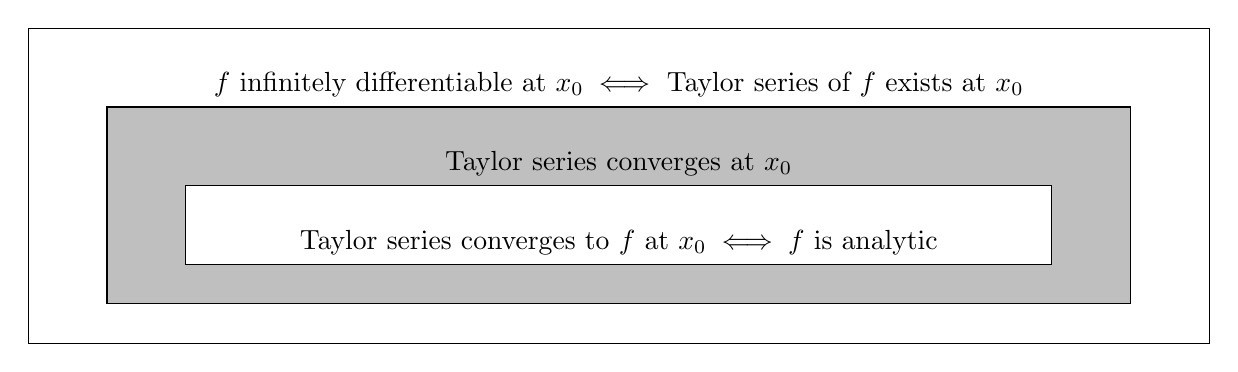
\begin{tikzpicture}
      \draw (-7.5,0) rectangle (7.5, 4);
      \draw[fill=lightgray] (-6.5, 0.5) rectangle (6.5, 3);
      \draw[fill=white] (-5.5, 1) rectangle (5.5, 2);
      \node[above] at (0, 1) {Taylor series converges to $f$ at $x_0 \iff f$ is analytic};
      \node[above] at (0, 2) {Taylor series converges at $x_0$};
      \node[above] at (0, 3) {$f$ infinitely differentiable at $x_0 \iff $ Taylor series of $f$ exists at $x_0$};
    \end{tikzpicture}
  \end{center}

  The following lemma proves why Taylor Polynomials are considered a "good" approximations to analytic functions. 

  \begin{lemma}[Infinitesimality of Functions with Vanishing Derivative up to Order $n$]
    Given a function $\varphi: E \longrightarrow \mathbb{R}$ defined on a closed interval $E$ with endpoint $x_0$, let its derivatives vanish up to order $n$ at $x_0$. That is
    \begin{equation}
      \varphi(x_0) = \varphi^\prime (x_0) = \ldots = \varphi^{(n)} (x_0) = 0
    \end{equation}
    Then, $\varphi = o\big((x - x_0)^n\big)$ as $x \rightarrow x_0$. 
  \end{lemma}
  \begin{proof}
    We prove by induction. For $n = 1$, the definition of differentiability states that 
    \begin{equation}
      \varphi(x) = \varphi^(x_0) + \varphi^\prime (x - x_0) + o(x - x_0) \text{ as } x \rightarrow x_0
    \end{equation}

    and so we have proved that 
    \begin{equation}
      \varphi(x_0) = \varphi^\prime (x_0) = 0 \implies \varphi(x) = o(x - x_0) \text{ as } x \rightarrow x_0
    \end{equation}

    Now, suppose this assertion has been proved for order $n = k - 1 \geq 1$. That is, we have shown that 
    \begin{equation}
      \varphi(x_0) = \ldots = \varphi^{(k-1)}(x_0) = 0 \implies \varphi= o\big((x - x_0)^{k-1}\big) \text{ as } x \rightarrow x_0
    \end{equation}

    Then we must show that this is valid for order $n = k \geq 2$. Assume that 
    \begin{equation}
      \varphi(x_0) = \varphi^\prime (x_0) = \ldots = \varphi^{(k)} (x_0) = 0
    \end{equation}

    We can see that this is equivalent to
    \begin{equation}
      (\varphi^\prime)^\prime (x_0) = (\varphi^\prime)^{(2)} (x_0) = \ldots = (\varphi^\prime)^{(k-1)} = 0
    \end{equation}

    and therefore by the induction assumption, we have
    \begin{equation}
      \varphi^\prime = o\big( (x - x_0)^{k-1}\big) \text{ as } x \rightarrow x_0
    \end{equation}
    which means that we can put it in form 
    \begin{equation}
      \varphi(x) = \alpha (x) (x - x_0)^{k-1} \text{ so that } \lim_{x \rightarrow x_0} \varphi(x) = \lim_{x \rightarrow x_0} \alpha(x) = 0
    \end{equation}

    From the mean value theorem and substituting what we have above, we get 
    \begin{align}
        \varphi(x) = \varphi(x) - \varphi(x_0) & = \varphi^\prime(\zeta) (x - x_0) \\
                                               & = \varphi (\zeta) (\zeta - x_0)^{k-1} (x - x_0)
    \end{align}

    where $\zeta \in (x_0, x)$. However, this implies that $|\zeta - x_0| < |x - x_0|$, and thus, as $x \rightarrow x_0$, $\zeta \rightarrow x_0$, which then makes $\alpha(\zeta) \rightarrow 0$. Since
    \begin{equation}
      |\varphi (x)| \leq |\alpha(\zeta)| |x - x_0|^{k-1} |x - x_0| = |\alpha(\zeta)| |x - x_0|^k
    \end{equation}

    This means that $\varphi(x)$ is bounded by function $|\alpha(\zeta)| |x - x_0|^k$, which is $o\big((x-x_0)^k\big)$, and so 
    \begin{equation}
      \varphi = o\big( (x - x_0)^k \big) \text{ as } x \rightarrow x_0
    \end{equation}
    By induction, this works for all orders $n$. 
  \end{proof}

  \begin{theorem}[Peano's Form of the Remainder]
    Given analytic function $f: E \longrightarrow \mathbb{R}$, a point $x_0 \in E$, and its $n$th order Taylor polynomial $P_n (x_0; x)$ around $x_0$, $P_n$ is a "good" approximation of $f$ in the fact that its error term is $o\big((x - x_0)^n\big)$. That is, 
    \begin{equation}
      f(x) = P_n (x_0; x) + o\big((x - x_0)^n \big) \text{ as } x \rightarrow x_0
    \end{equation}
    This equation where $r_n (x; x_0) = o\big((x - x_0)^n\big)$ is called the \textbf{Peano's form of the remainder}. 
  \end{theorem}
  \begin{proof}
    Since the Taylor polynomial $P_n (x_0; x)$ is constructed from the requirement that its derivatives up to order $n$ inclusive must coincide with the corresponding derivatives of $f$ at $x_0$, it follows that
    \begin{equation}
      r_n (x_0; x_0) \coloneqq f^{(k)} (x_0) - P_n^{(k)} (x_0; x_0) = 0 \text{ for } k = 0, 1, \ldots, n
    \end{equation}
    Using the previous lemma, a this means that $r_n (x; x_0) = o\big((x - x_0)^n\big)$ as $x \rightarrow x_0$. 
  \end{proof}

  \begin{theorem}[Lagrange Form of the Remainder]
    If $f: E \longrightarrow \mathbb{R}$ has derivatives of order $n+1$ on the open interval with endpoints $x_0$ and $x$, then 
    \begin{equation}
      f(x) = f(x_0) + \frac{f^\prime (x_0)}{1!} (x - x_0) + \ldots + \frac{f^{(n)}(x_0)}{n!} (x - x_0)^n + r_n (x; x_0)
    \end{equation}
    where 
    \begin{equation}
      r_n (x; x_0) = \frac{f^{(n+1)} (\zeta)}{(n+1)!} (x - x_0)^{n+1}
    \end{equation}
    This form is called \textbf{Taylor's formula with the Lagrange form of the remainder}. Furthermore, this form says that if $f^{(n+1)} (x)$ is bounded in a neighborhood of $x_0$, it also implies the formula
    \begin{equation}
      f(x) = f(x_0) + \frac{f^\prime (x_0)}{1!} (x - x_0) + \ldots + \frac{f^{(n)} (x_0)}{n!} (x - x_0)^n + O\big( (x - x_0)^{n+1} \big)
    \end{equation}
    Therefore, we can use this boundedness of $f^{(n+1)}$ to find the maximum error bound 
    \begin{equation}
      |r_n (x; x_0)|
    \end{equation}
    of $P_n (x; x_0)$. 
  \end{theorem}
  \begin{proof}
    It is a direct result from the lemma. This is actually a generalization of the mean value theorem but for higher orders. 
  \end{proof}

  \begin{corollary}[Table of Asymptotic Formulas for Elementary Functions]
    We write the Maclaurin series (Taylor series around $x = 0$) for elementary functions. Note that these error terms are $O(x^{n+1})$ (bounded compared to $x^{n+1}$) and $o(x^n)$ (infinitesimal compared to $x^n$). 
    \begin{align}
      e^x & = 1 + \frac{1}{1!} x + \frac{1}{2!} x^2 + \ldots + \frac{1}{n!} x^n + O(x^{n+1}) \\
      \cos{x} & = 1 - \frac{1}{2!} x^2 + \frac{1}{4!}x^4 - \ldots + \frac{(-1)^n}{(2n)!} x^{2n} + O(x^{2n+2}) \\
      \sin{x} & = x - \frac{1}{3!} x^3 + \frac{1}{5!}x^5 - \ldots + \frac{(-1)^n}{(2n+1)!} x^{2n+1} + O(x^{2n+3}) \\
      \cosh{x} & = 1 + \frac{1}{2!} x^2 + \frac{1}{4!} x^4 + \ldots + \frac{1}{(2n)!} x^{2n} + O(x^{2n+2}) \\
      \sinh{x} & = x + \frac{1}{3!} x^3 + \frac{1}{5!} x^5 + \ldots + \frac{1}{(2n+1)!} x^{2n+1} + O(x^{2n+3}) \\
      \ln{(1+x)} & = x - \frac{1}{2}x^2 + \frac{1}{3} x^3 - \ldots + \frac{(-1)^n}{n} x^n + O(x^{n+1}) \\
      (1 + x)^\alpha & = 1 + \frac{\alpha}{1!} x + \frac{\alpha(\alpha-1)}{2!} x^2 + \ldots + \frac{\alpha (\alpha-1) \ldots (\alpha - n + 1)}{n!} x^n + O(x^{n+1})
    \end{align}
  \end{corollary}

\subsection{Exercises}

  \begin{exercise}[Rudin 5.1]
    Let $f$ be defined for all real $x$, and suppose that
    \begin{equation}
      |f(x) - f(y)| \le (x - y)^2
    \end{equation}
    for all real $x$ and $y$. Prove that $f$ is constant.
  \end{exercise}
  \begin{solution}

  \end{solution}

  \begin{exercise}[Rudin 5.2]
    Suppose $f^\prime(x) > 0$ in $(a, b)$. Prove that $f$ is strictly increasing in $(a, b)$, and let $g$ be its inverse function. Prove that $g$ is differentiable, and that
    \begin{equation}
      g^\prime(f(x)) = \frac{1}{f^\prime(x)} \quad (a < x < b)
    \end{equation}
   .
  \end{exercise}
  \begin{solution}

  \end{solution}

  \begin{exercise}[Rudin 5.3]
    Suppose $g$ is a real function on $R^1$, with bounded derivative (say $|g^\prime| \le M$). Fix $\epsilon > 0$, and define $f(x) = x + \epsilon g(x)$. Prove that $f$ is one-to-one if $\epsilon$ is small enough. (A set of admissible values of $\epsilon$ can be determined which depends only on $M$.)
  \end{exercise}
  \begin{solution}

  \end{solution}

  \begin{exercise}[Rudin 5.4]
    If
    \begin{equation}
      C_0 + \frac{C_1}{2} + \dots + \frac{C_{n-1}}{n} + \frac{C_n}{n+1} = 0
    \end{equation}
    where $C_0, \dots, C_n$ are real constants, prove that the equation
    \begin{equation}
      C_0 + C_1 x + \dots + C_{n-1} x^{n-1} + C_n x^n = 0
    \end{equation}
    has at least one real root between 0 and 1.
  \end{exercise}
  \begin{solution}

  \end{solution}

  \begin{exercise}[Rudin 5.5]
    Suppose $f$ is defined and differentiable for every $x > 0$, and $f^\prime(x) \to 0$ as $x \to +\infty$. Put $g(x) = f(x + 1) - f(x)$. Prove that $g(x) \to 0$ as $x \to +\infty$.
  \end{exercise}
  \begin{solution}

  \end{solution}

  \begin{exercise}[Rudin 5.6]
    Suppose
    \begin{enumerate}
      \item[(a)] $f$ is continuous for $x \ge 0$,
      \item[(b)] $f^\prime(x)$ exists for $x > 0$,
      \item[(c)] $f(0) = 0$,
      \item[(d)] $f^\prime$ is monotonically increasing.
    \end{enumerate}
    Put
    \begin{equation}
      g(x) = \frac{f(x)}{x} \quad (x > 0)
    \end{equation}
    and prove that $g$ is monotonically increasing.
  \end{exercise}
  \begin{solution}

  \end{solution}

  \begin{exercise}[Rudin 5.7]
    Suppose $f^\prime(x), g^\prime(x)$ exist, $g^\prime(x) \ne 0$, and $f(x) = g(x) = 0$. Prove that
    \begin{equation}
      \lim_{t \to x} \frac{f(t)}{g(t)} = \frac{f^\prime(x)}{g^\prime(x)}
    \end{equation}
   . (This holds also for complex functions.)
  \end{exercise}
  \begin{solution}

  \end{solution}

  \begin{exercise}[Rudin 5.8]
    Suppose $f^\prime$ is continuous on $[a, b]$ and $\epsilon > 0$. Prove that there exists $\delta > 0$ such that
    \begin{equation}
      \left| \frac{f(t) - f(x)}{t - x} - f^\prime(x) \right| < \epsilon
    \end{equation}
    whenever $0 < |t - x| < \delta, a \le x \le b, a \le t \le b$. (This could be expressed by saying that $f$ is uniformly differentiable on $[a, b]$ if $f^\prime$ is continuous on $[a, b]$.) Does this hold for vector-valued functions too?
  \end{exercise}
  \begin{solution}

  \end{solution}

  \begin{exercise}[Rudin 5.9]
    Let $f$ be a continuous real function on $R^1$, of which it is known that $f^\prime(x)$ exists for all $x \ne 0$ and that $f^\prime(x) \to 3$ as $x \to 0$. Does it follow that $f^\prime(0)$ exists?
  \end{exercise}
  \begin{solution}

  \end{solution}

  \begin{exercise}[Rudin 5.10]
    Suppose $f$ and $g$ are complex differentiable functions on $(0, 1)$, $f(x) \to 0, g(x) \to 0, f^\prime(x) \to A, g^\prime(x) \to B$ as $x \to 0$, where $A$ and $B$ are complex numbers, $B \ne 0$. Prove that
    \begin{equation}
      \lim_{x \to 0} \frac{f(x)}{g(x)} = \frac{A}{B}
    \end{equation}
   . Compare with Example 5.18. \textit{Hint:}
    \begin{equation}
      \frac{f(x)}{g(x)} = \left\{ \frac{f(x)}{x} - A \right\} \cdot \frac{x}{g(x)} + A \cdot \frac{x}{g(x)}
    \end{equation}
   . Apply Theorem 5.13 to the real and imaginary parts of $f(x)/x$ and $g(x)/x$.
  \end{exercise}
  \begin{solution}

  \end{solution}

  \begin{exercise}[Rudin 5.11]
    Suppose $f$ is defined in a neighborhood of $x$, and suppose $f^{\prime\prime}(x)$ exists. Show that
    \begin{equation}
      \lim_{h \to 0} \frac{f(x + h) + f(x - h) - 2f(x)}{h^2} = f^{\prime\prime}(x)
    \end{equation}
   . Show by an example that the limit may exist even if $f^{\prime\prime}(x)$ does not. \textit{Hint:} Use Theorem 5.13.
  \end{exercise}
  \begin{solution}

  \end{solution}

  \begin{exercise}[Rudin 5.12]
    If $f(x) = |x|^3$, compute $f^\prime(x), f^{\prime\prime}(x)$ for all real $x$, and show that $f^{(3)}(0)$ does not exist.
  \end{exercise}
  \begin{solution}

  \end{solution}

  \begin{exercise}[Rudin 5.13]
    Suppose $a$ and $c$ are real numbers, $c > 0$, and $f$ is defined on $[-1, 1]$ by
    \begin{equation}
      f(x) = 
      \begin{cases}
        x^a \sin(|x|^{-c}) & (\text{if } x \ne 0), \\
        0 & (\text{if } x = 0)
      \end{cases}
    \end{equation}
   . Prove the following statements:
    \begin{enumerate}
      \item[(a)] $f$ is continuous if and only if $a > 0$.
      \item[(b)] $f^\prime(0)$ exists if and only if $a > 1$.
      \item[(c)] $f^\prime$ is bounded if and only if $a \ge 1 + c$.
      \item[(d)] $f^\prime$ is continuous if and only if $a > 1 + c$.
      \item[(e)] $f^{\prime\prime}(0)$ exists if and only if $a > 2 + c$.
      \item[(f)] $f^{\prime\prime}$ is bounded if and only if $a \ge 2 + 2c$.
      \item[(g)] $f^{\prime\prime}$ is continuous if and only if $a > 2 + 2c$.
    \end{enumerate}
  \end{exercise}
  \begin{solution}

  \end{solution}

  \begin{exercise}[Rudin 5.14]
    Let $f$ be a differentiable real function defined in $(a, b)$. Prove that $f$ is convex if and only if $f^\prime$ is monotonically increasing. Assume next that $f^{\prime\prime}(x)$ exists for every $x \in (a, b)$, and prove that $f$ is convex if and only if $f^{\prime\prime}(x) \ge 0$ for all $x \in (a, b)$.
  \end{exercise}
  \begin{solution}

  \end{solution}

  \begin{exercise}[Rudin 5.15]
    Suppose $a \in R^1$, $f$ is a twice-differentiable real function on $(a, \infty)$, and $M_0, M_1, M_2$ are the least upper bounds of $|f(x)|, |f^\prime(x)|, |f^{\prime\prime}(x)|$, respectively, on $(a, \infty)$. Prove that
    \begin{equation}
      M_1^2 \le 4M_0 M_2
    \end{equation}
   . \textit{Hint:} If $h > 0$, Taylor's theorem shows that
    \begin{equation}
      f^\prime(x) = \frac{1}{2h} [f(x + 2h) - f(x)] - hf^{\prime\prime}(\xi)
    \end{equation}
    for some $\xi \in (x, x + 2h)$. Hence
    \begin{equation}
      |f^\prime(x)| \le hM_2 + \frac{M_0}{h}
    \end{equation}
   . To show that $M_1^2 = 4M_0 M_2$ can actually happen, take $a = -1$, define
    \begin{equation}
      f(x) = 
      \begin{cases}
        2x^2 - 1 & (-1 < x < 0), \\
        \frac{x^2 - 1}{x^2 + 1} & (0 \le x < \infty)
      \end{cases}
    \end{equation}
    and show that $M_0 = 1, M_1 = 4, M_2 = 4$. Does $M_1^2 \le 4M_0 M_2$ hold for vector-valued functions too?
  \end{exercise}
  \begin{solution}

  \end{solution}

  \begin{exercise}[Rudin 5.16]
    Suppose $f$ is twice-differentiable on $(0, \infty)$, $f^{\prime\prime}$ is bounded on $(0, \infty)$, and $f(x) \to 0$ as $x \to \infty$. Prove that $f^\prime(x) \to 0$ as $x \to \infty$. \textit{Hint:} Let $a \to \infty$ in Exercise 15.
  \end{exercise}
  \begin{solution}

  \end{solution}

  \begin{exercise}[Rudin 5.17]
    Suppose $f$ is a real, three times differentiable function on $[-1, 1]$, such that
    \begin{equation}
      f(-1) = 0, \quad f(0) = 0, \quad f(1) = 1, \quad f^\prime(0) = 0
    \end{equation}
   . Prove that $f^{(3)}(x) \ge 3$ for some $x \in (-1, 1)$. Note that equality holds for $\frac{1}{2}(x^3 + x^2)$. \textit{Hint:} Use Theorem 5.15, with $\alpha = 0$ and $\beta = \pm 1$, to show that there exist $s \in (0, 1)$ and $t \in (-1, 0)$ such that $f^{(3)}(s) + f^{(3)}(t) = 6$.
  \end{exercise}
  \begin{solution}

  \end{solution}

  \begin{exercise}[Rudin 5.18]
    Suppose $f$ is a real function on $[a, b]$, $n$ is a positive integer, and $f^{(n-1)}$ exists for every $t \in [a, b]$. Let $\alpha, \beta$, and $P$ be as in Taylor's theorem (5.15). Define
    \begin{equation}
      Q(t) = \frac{f(t) - f(\beta)}{t - \beta}
    \end{equation}
    for $t \in [a, b], t \ne \beta$, differentiate $f(t) - f(\beta) = (t - \beta)Q(t)$ $n-1$ times at $t = \alpha$, and derive the following version of Taylor's theorem:
    \begin{equation}
      f(\beta) = P(\beta) + \frac{Q^{(n-1)}(\alpha)}{(n-1)!} (\beta - \alpha)^n
    \end{equation}
   .
  \end{exercise}
  \begin{solution}

  \end{solution}

  \begin{exercise}[Rudin 5.19]
    Suppose $f$ is defined in $(-1, 1)$ and $f^\prime(0)$ exists. Suppose $-1 < \alpha_n < \beta_n < 1$, $\alpha_n \to 0$, and $\beta_n \to 0$ as $n \to \infty$. Define the difference quotients
    \begin{equation}
      D_n = \frac{f(\beta_n) - f(\alpha_n)}{\beta_n - \alpha_n}
    \end{equation}
   . Prove the following statements:
    \begin{enumerate}
      \item[(a)] If $\alpha_n < 0 < \beta_n$, then $\lim D_n = f^\prime(0)$.
      \item[(b)] If $0 < \alpha_n < \beta_n$ and $\{\beta_n/(\beta_n - \alpha_n)\}$ is bounded, then $\lim D_n = f^\prime(0)$.
      \item[(c)] If $f^\prime$ is continuous in $(-1, 1)$, then $\lim D_n = f^\prime(0)$.
    \end{enumerate}
    Give an example in which $f$ is differentiable in $(-1, 1)$ (but $f^\prime$ is not continuous at 0) and in which $\alpha_n, \beta_n$ tend to 0 in such a way that $\lim D_n$ exists but is different from $f^\prime(0)$.
  \end{exercise}
  \begin{solution}

  \end{solution}

  \begin{exercise}[Rudin 5.22]
    Suppose $f$ is a real function on $(-\infty, \infty)$. Call $x$ a \textit{fixed point} of $f$ if $f(x) = x$.
    \begin{enumerate}
      \item[(a)] If $f$ is differentiable and $f^\prime(t) \ne 1$ for every real $t$, prove that $f$ has at most one fixed point.
      \item[(b)] Show that the function $f$ defined by
        \begin{equation}
          f(t) = t + (1 + e^t)^{-1}
        \end{equation}
        has no fixed point, although $0 < f^\prime(t) < 1$ for all real $t$.
      \item[(c)] However, if there is a constant $A < 1$ such that $|f^\prime(t)| \le A$ for all real $t$, prove that a fixed point $x$ of $f$ exists, and that $x = \lim x_n$, where $x_1$ is an arbitrary real number and $x_{n+1} = f(x_n)$ for $n = 1, 2, 3, \dots$.
      \item[(d)] Show that the process described in (c) can be visualized by the zig-zag path $(x_1, x_2) \to (x_2, x_2) \to (x_2, x_3) \to (x_3, x_3) \to (x_3, x_4) \to \dots$. 
    \end{enumerate}
  \end{exercise}
  \begin{solution}

  \end{solution}

  \begin{exercise}[Rudin 5.23]
    The function $f$ defined by
    \begin{equation}
      f(x) = \frac{x^3 + 1}{3}
    \end{equation}
    has three fixed points, say $\alpha, \beta, \gamma$, where
    \begin{equation}
      -2 < \alpha < -1, \quad 0 < \beta < 1, \quad 1 < \gamma < 2
    \end{equation}
   . For arbitrarily chosen $x_1$, define $\{x_n\}$ by setting $x_{n+1} = f(x_n)$.
    \begin{enumerate}
      \item[(a)] If $x_1 < \alpha$, prove that $x_n \to -\infty$ as $n \to \infty$.
      \item[(b)] If $\alpha < x_1 < \gamma$, prove that $x_n \to \beta$ as $n \to \infty$.
      \item[(c)] If $\gamma < x_1$, prove that $x_n \to +\infty$ as $n \to \infty$.
    \end{enumerate}
    Thus $\beta$ can be located by this method, but $\alpha$ and $\gamma$ cannot.
  \end{exercise}
  \begin{solution}

  \end{solution}

  \begin{exercise}[Rudin 5.25]
    Suppose $f$ is twice differentiable on $[a, b]$, $f(a) < 0, f(b) > 0, f^\prime(x) \ge \delta > 0$, and $0 \le f^{\prime\prime}(x) \le M$ for all $x \in [a, b]$. Let $\xi$ be the unique point in $(a, b)$ at which $f(\xi) = 0$. Complete the details in the following outline of \textit{Newton's method} for computing $\xi$.
    \begin{enumerate}
      \item[(a)] Choose $x_1 \in (\xi, b)$, and define $\{x_n\}$ by
        \begin{equation}
          x_{n+1} = x_n - \frac{f(x_n)}{f^\prime(x_n)}
        \end{equation}
       . Interpret this geometrically, in terms of a tangent to the graph of $f$.
      \item[(b)] Prove that $x_{n+1} < x_n$ and that $\lim x_n = \xi$.
      \item[(c)] Use Taylor's theorem to show that
        \begin{equation}
          x_{n+1} - \xi = \frac{f^{\prime\prime}(t_n)}{2f^\prime(x_n)}(x_n - \xi)^2
        \end{equation}
        for some $t_n \in (\xi, x_n)$.
      \item[(d)] If $A = M/2\delta$, deduce that
        \begin{equation}
          0 \le x_{n+1} - \xi \le \frac{1}{A} [A(x_1 - \xi)]^{2^n}
        \end{equation}
       .
      \item[(e)] Show that Newton's method amounts to finding a fixed point of the function $g$ defined by
        \begin{equation}
          g(x) = x - \frac{f(x)}{f^\prime(x)}
        \end{equation}
       . How does $g^\prime(x)$ behave for $x$ near $\xi$?
      \item[(f)] Put $f(x) = x^{1/3}$ on $(-\infty, \infty)$ and try Newton's method. What happens?
    \end{enumerate}
  \end{exercise}
  \begin{solution}

  \end{solution}

  \begin{exercise}[Rudin 5.26]
    Suppose $f$ is differentiable on $[a, b], f(a) = 0$, and there is a real number $A$ such that $|f^\prime(x)| \le A|f(x)|$ on $[a, b]$. Prove that $f(x) = 0$ for all $x \in [a, b]$. \textit{Hint:} Fix $x_0 \in [a, b]$, let
    \begin{equation}
      M_0 = \sup|f(x)|, \quad M_1 = \sup|f^\prime(x)|
    \end{equation}
    for $a \le x \le x_0$. For any such $x$, $|f(x)| \le M_1(x_0 - a) \le A(x_0 - a)M_0$. Hence $M_0 = 0$ if $A(x_0 - a) < 1$. That is, $f = 0$ on $[a, x_0]$. Proceed.
  \end{exercise}
  \begin{solution}

  \end{solution}

  \begin{exercise}[Rudin 5.27]
    Let $\phi$ be a real function defined on a rectangle $R$ in the plane, given by $a \le x \le b, \alpha \le y \le \beta$. A \textit{solution of the initial-value problem}
    \begin{equation}
      y^\prime = \phi(x, y), \quad y(a) = c \quad (\alpha \le c \le \beta)
    \end{equation}
    is, by definition, a differentiable function $f$ on $[a, b]$ such that $f(a) = c, \alpha \le f(x) \le \beta$, and
    \begin{equation}
      f^\prime(x) = \phi(x, f(x)) \quad (a \le x \le b)
    \end{equation}
   . Prove that such a problem has at most one solution if there is a constant $A$ such that
    \begin{equation}
      |\phi(x, y_2) - \phi(x, y_1)| \le A|y_2 - y_1|
    \end{equation}
    whenever $(x, y_1) \in R$ and $(x, y_2) \in R$. \textit{Hint:} Apply Exercise 26 to the difference of two solutions. Note that this uniqueness theorem does not hold for the initial-value problem $y^\prime = y^{1/2}, y(0) = 0$, which has two solutions: $f(x) = 0$ and $f(x) = x^2/4$. Find all other solutions.
  \end{exercise}
  \begin{solution}

  \end{solution}

  \begin{exercise}[Rudin 5.28]
    Formulate and prove an analogous uniqueness theorem for systems of differential equations of the form
    \begin{equation}
      y^\prime_j = \phi_j(x, y_1, \dots, y_k), \quad y_j(a) = c_j \quad (j = 1, \dots, k)
    \end{equation}
   . Note that this can be rewritten in the form
    \begin{equation}
      \mathbf{y}^\prime = \mathbf{\Phi}(x, \mathbf{y}), \quad \mathbf{y}(a) = \mathbf{c}
    \end{equation}
    where $\mathbf{y} = (y_1, \dots, y_k)$ ranges over a $k$-cell, $\mathbf{\Phi}$ is the mapping of a $(k+1)$-cell into the Euclidean $k$-space whose components are the functions $\phi_1, \dots, \phi_k$, and $\mathbf{c}$ is the vector $(c_1, \dots, c_k)$. Use Exercise 26, for vector-valued functions.
  \end{exercise}
  \begin{solution}

  \end{solution}

  \begin{exercise}[Rudin 5.29]
    Specialize Exercise 28 by considering the system
    \begin{equation}
      y^\prime_j = y_{j+1} \quad (j = 1, \dots, k-1)
    \end{equation}
   ,
    \begin{equation}
      y^\prime_k = f(x) - \sum_{j=1}^k g_j(x) y_j
    \end{equation}
   , where $f, g_1, \dots, g_k$ are continuous real functions on $[a, b]$, and derive a uniqueness theorem for solutions of the equation
    \begin{equation}
      y^{(k)} + g_k(x)y^{(k-1)} + \dots + g_2(x)y^\prime + g_1(x)y = f(x)
    \end{equation}
   , subject to initial conditions
    \begin{equation}
      y(a) = c_1, \quad y^\prime(a) = c_2, \quad \dots, \quad y^{(k-1)}(a) = c_k
    \end{equation}
   .
  \end{exercise}
  \begin{solution}

  \end{solution}
  
  \begin{exercise}[Math 531 Spring 2025, PS7.5]
    Coming back to Problem 1 above, assume that $f$ is differentiable on $[0, 1]$ and that $|f'(x)| \leq M$ for every $x \in [0, 1]$. Prove that we can take $\delta(\epsilon) = \frac{\epsilon}{M}$.
  \end{exercise}
  \begin{solution}

  \end{solution}

  \begin{exercise}[Math 531 Spring 2025, PS7.7]
    Suppose that $f : [0, 2] \to [0, 2]$ is twice differentiable. Suppose $f(0) = 0$, $f(1) = 1$, and $f(2) = 2$. Prove that there exists $c \in (0, 2)$ so that $f''(c) = 0$.
  \end{exercise}
  \begin{solution}

  \end{solution}

  \begin{exercise}[Math 531 Spring 2025, PS7.8]
    Suppose that $f$ is differentiable on $[0, 1]$ satisfies:
    \begin{equation}
      f'(x) = f(x).
    \end{equation}
    
    \begin{itemize}
      \item Prove that $f$ is automatically infinitely differentiable.
      
      \item Let $M = \max\{f(x) : x \in [0, 1]\}$. Why does $M$ exist? Similarly, let $M(\epsilon) = \max\{|f(x)| : x \in [0, \epsilon]\}$.
      
      \item Prove that for all $x \in [0, \epsilon]$, we have that
      \begin{equation}
        |f(x)| \leq M(\epsilon)x + |f(0)|.
      \end{equation}
      
      \item Deduce that if $f(0) = 0$, we have that
      \begin{equation}
        M\left(\frac{1}{2}\right) = 0.
      \end{equation}
      Similarly, deduce that $M(c) = 0$ for all $c \in [0, 1]$.
      
      \item What you have just proved is that if $f'(x) = f(x)$ while $f(0) = 0$, it follows that $f(x) = 0$ for all $x$.
      
      \item Assume that $E : \mathbb{R} \to [0, \infty)$ is differentiable and
      \begin{equation}
        |E'(t)| \leq CE(t).
      \end{equation}
      Prove that if $E(0) = 0$, then $E(t) = 0$ for all $t$.
    \end{itemize}
  \end{exercise}
  \begin{solution}

  \end{solution}

  \begin{exercise}[Math 531 Spring 2025, PS8.1]
    Prove that if $f : [0, 1] \to \mathbb{R}$ is differentiable and $f' > 0$ on $[0, 1]$, then $f$ is strictly increasing on $[0, 1]$.
  \end{exercise}
  \begin{solution}

  \end{solution}

  \begin{exercise}[Math 531 Spring 2025, PS8.2]
    Explain why if $x(t)$ represents the position of a particle at time $t$, $x'(t)$ is called the velocity of the particle, $x''(t)$ is called its acceleration, and $x'''(t)$ is called its jerk.
  \end{exercise}
  \begin{solution}

  \end{solution}

  \begin{exercise}[Math 531 Spring 2025, PS8.3]
    A function $f : \mathbb{R} \to \mathbb{R}$ is said to be $T$ periodic if $f(t + T) = f(t)$, for all $t \in \mathbb{R}$. Now, given a function $\tilde{f}$ defined on $[0, T)$, we can always extend $\tilde{f}$ to be $T$ periodic in the following way. First, we can write
    \begin{equation}
      \mathbb{R} = \bigcup_{n\in\mathbb{Z}} [nT,(n + 1)T).
    \end{equation}
    Then define for $t \in [nT,(n + 1)T)$ :
    \begin{equation}
      f(t) = \tilde{f}(t - nT).
    \end{equation}
    
    \begin{itemize}
      \item Show that $f$ defined this way is $T$ periodic.
      \item Suppose $\tilde{f}$ is continuous on $[0, T)$. Does this mean that its extension $f$ will also be continuous on $\mathbb{R}$? What condition do you have to add?
      \item Suppose $\tilde{f}$ is continuously differentiable on $[0, T)$. What conditions do you have to put on $\tilde{f}$ to ensure that $f$ is continuously differentiable? How about $k$-times continuously differentiable?
    \end{itemize}
  \end{exercise}
  \begin{solution}

  \end{solution}

  \begin{exercise}[Math 531 Spring 2025, PS8.4]
    Assume $f : \mathbb{R} \to \mathbb{R}$ is differentiable and $|f'(x)| \leq \frac{1}{1+x^2}$. Prove that
    \begin{equation}
      \lim_{x\to\infty}f(x)
    \end{equation}
    exists. You are not allowed to use integration. Hint: How do you prove convergence without knowing what the limit is?
  \end{exercise}
  \begin{solution}

  \end{solution}

  \begin{exercise}[Math 531 Spring 2025, PS8.5]
    In a previous homework assignment, we defined the function
    \begin{equation}
      E(x) = \sum_{n=0}^{\infty} \frac{x^n}{n!}.
    \end{equation}
    
    We proved it is continuous, satisfies $E(z+w) = E(z)E(w)$ for all $z, w \in \mathbb{C}$, and then deduced that for all $x \in \mathbb{R}$, we have that $E(x) = e^x$.
    
    \begin{itemize}
      \item Prove that $E'(0) = 1$. Hint: write $\frac{H(x)-H(0)}{x} = \frac{1}{x} \sum_{n=1}^{\infty} \frac{x^n}{n!} = \sum_{n=1}^{\infty} \frac{x^{n-1}}{n!}$. Then prove that
      \begin{equation}
        \lim_{x\to 0} \sum_{n=1}^{\infty} \frac{x^{n-1}}{n!} = 1.
      \end{equation}
      
      \item By studying the difference quotient, prove that $E'(x) = E(x)$ for all $x \in \mathbb{R}$. This is much easier than the preceding point.
      
      \item Prove that $\lim_{x\to\infty} E(x) = \infty$ and $\lim_{x\to-\infty} E(x) = 0$.
      
      \item Prove that $E : (-\infty, \infty) \to (0, \infty)$ is 1-1 and onto.
      
      \item Let $L = E^{-1}: (0, \infty) \to (-\infty, \infty)$. Prove that
      \begin{equation}
        L'(t) = \frac{1}{t},
      \end{equation}
      for all $t \in (0, \infty)$.
    \end{itemize}
  \end{exercise}
  \begin{solution}

  \end{solution}

  \begin{exercise}[Math 531 Spring 2025, PS8.6]
    For each $k \in \mathbb{N}$, consider $\sum_{j=1}^N j^k$. It turns out that this can be expressed as a polynomial of degree $k + 1$ in $N$. For example,
    \begin{equation}
      \sum_{j=1}^N j^0 = N,
    \end{equation}
    is a polynomial of degree 1 in $N$. Similarly,
    \begin{equation}
      \sum_{j=1}^N j = \frac{N(N + 1)}{2} = \frac{N^2}{2} + \frac{N}{2},
    \end{equation}
    is a polynomial of degree 2 in $N$. If we write:
    \begin{equation}
      \sum_{j=1}^N j^k = a_0 + a_1N + a_2N^2 + ... + a_{k+1}N^{k+1},
    \end{equation}
    what is the value of $a_{k+1}$? Hint: divide by $N^{k+1}$ and take the limit as $N \to \infty$.
  \end{exercise}
  \begin{solution}

  \end{solution}

  \begin{exercise}[Math 531 Spring 2025, PS9.3]
    Assume we have a twice differentiable function $f : [0, \infty) \to \mathbb{R}$. Assume that $f''(x) > 0$ for all $x \in [0, \infty)$, while $f'(0) \geq 0$. Prove that $\lim_{x\to\infty} f(x) = +\infty$.
  \end{exercise}
  \begin{solution}

  \end{solution}

  \begin{exercise}[Math 531 Spring 2025, PS9.4]
    We proved that the function $E : \mathbb{C} \to \mathbb{C}$ defined by:
    \begin{equation}
      E(z) = \sum_{k=0}^{\infty} \frac{z^k}{k!}
    \end{equation}
    satisfies $E(z + w) = E(z)E(w)$. Let us now investigate the real and imaginary parts of $E(it)$, where $t \in \mathbb{R}$. Let us call the real part $C(t)$ and the imaginary part $S(t)$.
    \begin{itemize}
      \item Prove that $E(\overline{z}) = \overline{E(z)}$, for every $z \in \mathbb{C}$.
      \item Deduce that $|E(it)| = 1$ for all $t \in \mathbb{R}$ and thus:
      \begin{equation}
        C(t)^2 + S(t)^2 = 1,
      \end{equation}
      for all $t \in \mathbb{R}$.
      \item Prove that $C(-t) = C(t)$ for all $t$ and that $S(-t) = -S(t)$ for all $t$.
      \item Prove that $C(0) = 1$ and $S(0) = 0$, while $C'(t) = -S(t)$ and $S'(t) = C(t)$, for all $t \in \mathbb{R}$.
      \item Deduce that $C''(t) = -C(t)$ and prove that there must be some $t > 0$ for which $C(t) = 0$. (Hint: Use Problem 3)
      \item Prove that there is a smallest $t_* > 0$ for which $C(t_*) = 0$.
      \item Define $\pi = 2t_*$ so that $C(\frac{\pi}{2}) = 0$. Since $S$ is increasing on $[0, t_*]$, deduce that $S(\frac{\pi}{2}) = 1$.
      \item Now use the formula $E(z + w) = E(z)E(w)$ to deduce that
      \begin{equation}
        C(t + 2\pi) = C(t), \quad S(t + 2\pi) = S(t),
      \end{equation}
      for all $t \in \mathbb{R}$.
      \item It is now reasonable to unveil that $C$ and $S$ are none other but our old friends: $\cos$ and $\sin$.
    \end{itemize}
  \end{exercise}
  \begin{solution}

  \end{solution}

